\documentclass[12pt]{beamer}

%%%%%%%%%%%%%%%%%%% Theme

\usetheme{metropolis}

%%%%%%%%%%%%%%%%%%% Packages

\usepackage[english]{babel}
\usepackage{packages/sleek-beamer}

%%%%%%%%%%%%%%%%%%% Bibliography

\addbibresource{./resources/bib/references.bib}

%%%%%%%%%%%%%%%%%%% Titlepage

\title{Semantic Data}
\subtitle{Ontology of the University of Liège}
\author{Yann Claes, Gaspard Lambrechts and François Rozet}
\institute{University of Liège}
\date{\today}
\titlelogo{./resources/pdf/logo.pdf}
\framelogo{./resources/pdf/logo.pdf}

%%%%%%%%%%%%%%%%%%%

\begin{document}

\maketitle

\section{Ontology presentation}

\begin{frame}{Imported Ontologies}
    In our \texttt{uliege} ontology, we imported the ontology \href{https://www.w3.org/2006/time}{\texttt{time}}.
\end{frame}

\begin{frame}{Ontology presentation}
    Our ontology articulates around 5 main classes:
    \begin{itemize}
        \item \texttt{Agent}, containing anything with a \alert{name} that can \alert{act}
        \item \texttt{Course}, covering the concept of a \alert{course}
        \item \texttt{Document}, referring to any \alert{official} document that can be \alert{published}
        \item \texttt{Event}, containing anything that \alert{happens} in time
        \item \texttt{Place}, covering the \alert{spatial} domain
    \end{itemize}
\end{frame}

\begin{frame}
    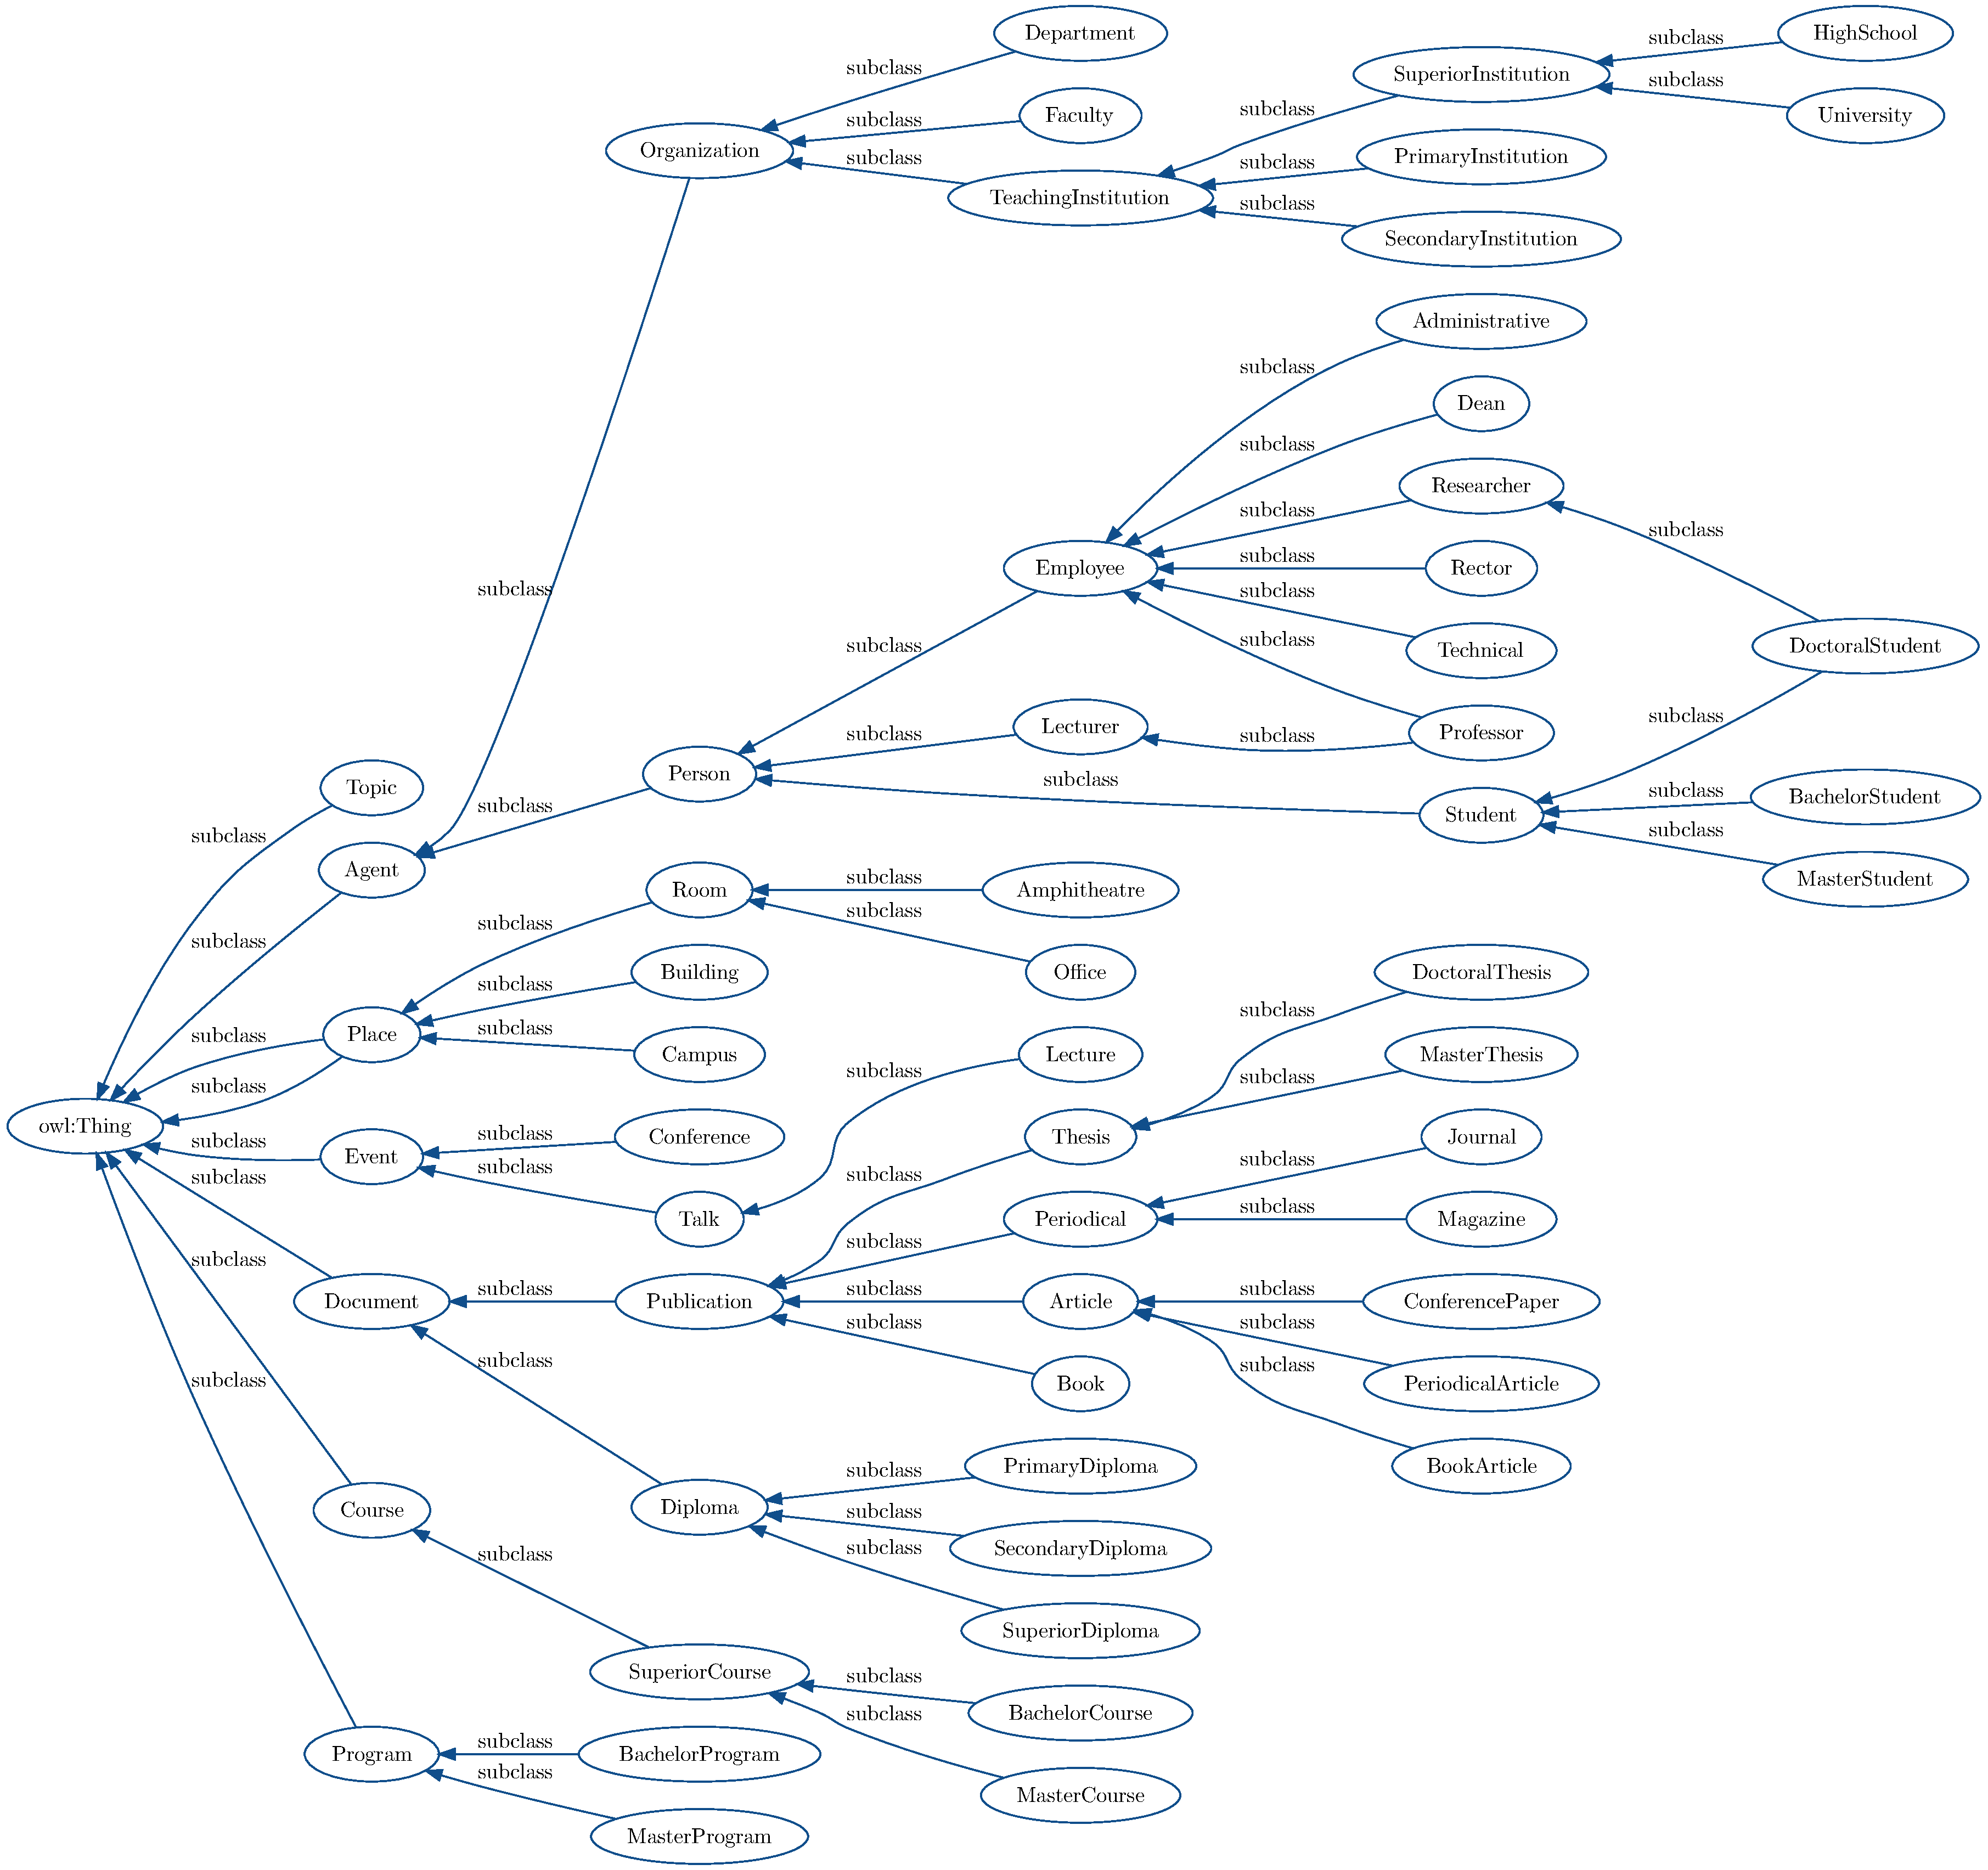
\includegraphics[height=.99\paperheight]{resources/pdf/class_hierarchy.pdf}
\end{frame}

\begin{frame}{Ontology presentation}
    We tried to satisfy the \alert{required} expectations of the guidelines, \emph{i.e.} modeling :
    \begin{itemize}
        \item Courses, programs and roles (student, professor, rector, etc.)
        \item The main components of a university (faculties, departments, campuses, etc.)
        \item Relate to other institutions and education levels (high schools, primary and secondary education) % Even though we could have populated them a little bit more
    \end{itemize}
\end{frame}

\begin{frame}{Ontology presentation}
    On top of that, we tried to add sufficient \alert{complexity} or ramifications in our classes definition.
    
    For that purpose, we used, \emph{where appropriate}, role restrictions, equivalent classes definitions (with intersections, unions, etc.)
\end{frame}

\begin{frame}[allowframebreaks]{Limitations of the ontology}
    \begin{itemize}
        \item We wanted to include some axioms of the type $$\forall x, y, z \quad P_1(x, y) \wedge P_2(y, z) \Rightarrow P_3(x, z), $$ but unfortunately, it was not possible.
        
        For instance, we wanted to introduce the axiom
        \begin{align*}
            \forall x, y, z \quad & followsCourse(x, y) \wedge hasAsPrerequisite(y, z) \\
            & \Rightarrow hasPassed(x, z)
        \end{align*}
    
        \item Our ontology corresponds to a snapshot in time. We haven't represented relations such has \texttt{wasRegisteredAt} or \texttt{wasStudent}.
        
        \item It is not possible to infer that a \texttt{Lecture} was given in a specific day because it is positioned in time only by its starting and ending date-time and also because it is not possible to perform \alert{arithmetic} inference in OWL. \\[0.5em]
                
        For instance, it is not possible to imply that \enquote{2020-05-06T09:00:00} is within \enquote{2020-05-06}.
    \end{itemize}
\end{frame}

\section{Population}

\begin{frame}{Populating the ontology}
    When \alert{populating} our ontology, we tried to create instances for as many classes as possible, if they were considered \alert{relevant}.
    
    Hence, some subclasses, such as \texttt{PrimaryInstitution}, \texttt{Periodical} or \texttt{Book}, have no corresponding instances.
\end{frame}

\begin{frame}{Populating the ontology}
    Furthermore, when creating the individuals, we tried to instantiate them from particular \alert{classes} and to assign them particular \alert{properties} in order to have interesting \alert{inferences} to retrieve.
    
    For example, the course \emph{Semantic Data} was asserted to be \emph{included in} the \emph{Master of Data Science and Engineering}. Hence, he was inferred to be a \emph{Master Course}.
\end{frame}

\section{Competency questions}

\begin{frame}[allowframebreaks]{Examples of competency questions}
    \footnotesize{
        \begin{itemize}
            \item Which students follow a course where at least one lecture has been given by Pr. Binot ?
            \item Which papers have been written by a certain student's professors ?
            \item Which students were following a lecture that started at 9am on 2020-05-06 ?
            \item Is the office of a professor located in a certain building / campus ?
            \item Which students have not been encoded as having attended all lectures of the courses they follow ? \emph{Note: in the OWA, we can't infer that these students have \alert{not} attended}
            
            \item Which students follow courses for which they are not encoded as having passed all the prerequisites ? \emph{Note: idem.}
            
            \item Which students follow courses taught by a professor that has written publications about the topic \emph{Electrical Power Systems} ?
            \item Which students are enrolled in a master program but already have a superior diploma ?
            
            \item For all students enrolled at the university of Liege, do they have a secondary diploma ? \emph{Note: answer is always yes thanks to some axioms.}
            
            \item Get all the persons that have their office in the same building. 
        \end{itemize}
    }
\end{frame}

\begin{frame}[standout]
  Let's move to the demonstration !
\end{frame}

\end{document}
